\section{Durchführung}
\label{sec:Durchführung}

Ein schematischer Aufbau ist in Abbildung \ref{fig:Aufbau} dargestellt. 

\begin{figure}
  \centering
  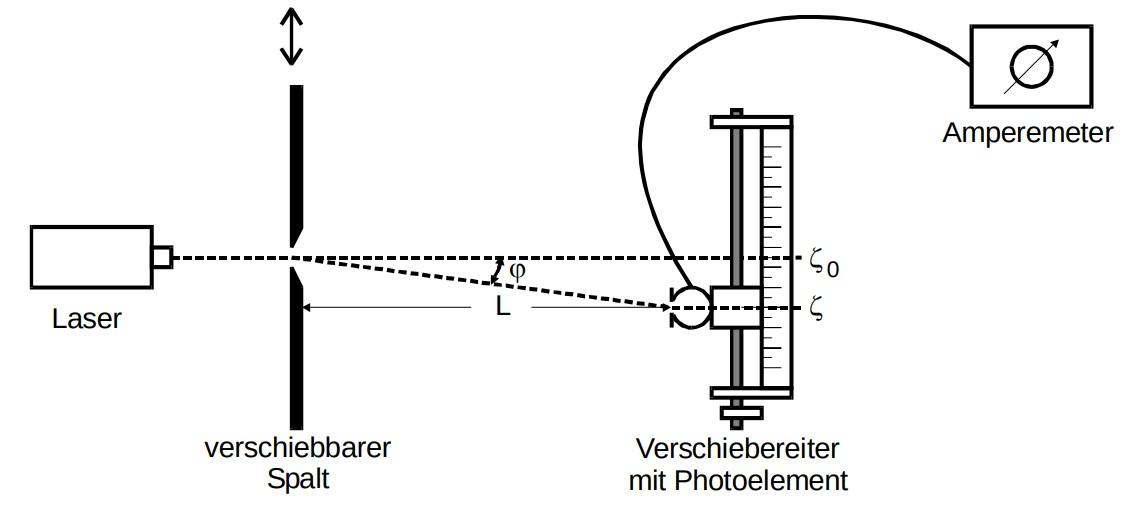
\includegraphics[scale=0.3]{content/Aufbau.jpg}
  \caption{Versuchsanordnung zur Abmessung einer Beugungsfigur. [1]}
  \label{fig:Aufbau}
\end{figure}

Zunächst wird die Strecke $L$ ausgemessen, die den Abstand zwischen dem Spalt und dem Photoelement angibt. 
Anschließend wird der erste Einzelspalt untersucht. Es ist darauf zu achten, dass vor jeder Messung 
bereits ein Strom $I_\text{Dunkel}$ gemessen werden muss, da das Photoelement auch im unbeleuchteten 
Zustand eine Intensität wahrnimmt. Dazu wird das Photoelement mit einem kalten lichtundurchlässigem Gegenstand 
abgedeckt und daraufhin der Dunkelstrom $I_\text{Dunkel}$ notiert. 
Für die eigentliche Intensitätsmessung wird der Gegenstand wieder entfernt und der angezeigte Strom $I$ notiert. \\
Das Photoelement wird nach diesen beiden Messungen weiter verschoben und die nächsten Messungen werden 
durchgeführt. In der Nähe des Hauptmaximums wird das Photoelement in $\SI{0.25}{\milli\meter}$ Schritten bewegt, weiter 
außen in $\SI{0.5}{\milli\meter}$ bzw. $\SI{1}{\milli\meter}$ Schritten. Aus dieser Messung ergeben sich insgesamt 
Datentripel bestehend aus der Verschiebung $x$ des Photoelements, des Dunkelstroms $I_\text{Dunkel}$ und $I$. \\
Insgesamt wird das Photoelement in beide Richtung des Hauptmaximas um $\SI{25}{\milli\meter}$ verschoben. \\
Der zweite Einzelspalt und der Doppelspalt werden analog vermessen. \\
Als letzter Schritt werden die Spalte mit einem Mikroskop untersucht. Dazu wird zunächst ein Lineal mit dem Mikroskop betrachtet, 
um dessen Vergößerung bestimmen zu können. Anschließend werden die Breiten $b$ der Einzelspalte und des Doppelspalts, 
sowie der Spaltabstand $s$ des Letzteren bestimmt und alle Werte notiert.  
